\documentclass{article}

\usepackage{listings}
\usepackage{color}
\usepackage{courier}
\usepackage{amsmath}
\usepackage{graphicx}
\usepackage{float}
\usepackage[spanish]{babel}
\usepackage[utf8]{inputenc}
\usepackage{mleftright}
\usepackage{csvsimple}

\newcommand{\lnn}[1]{%
	\ln\left(#1\right)%
}

\newcommand{\lnb}[1]{%
	\ln\mleft(#1\mright)%
}


\title{PEC III - Física Computacional II}
\date{12-11-2023}
\author{Arturo Felipe Albacete Fernández}



\lstset{
	basicstyle=\footnotesize\ttfamily,
	breaklines=true,
	frame=tb,
	tabsize=4,
	columns=fixed,
	showstringspaces=false,
	showtabs=false,
	keepspaces,
	commentstyle=\color{red},
	keywordstyle=\color{blue}
}
\lstset{frame=single}


\begin{document}

% titulo
\maketitle
\newpage

% TOC
\tableofcontents
\newpage

% intro
%
% Introducción
%

\section{Introducción}

\paragraph{}
En este documento se encuentran redactadas las respuestas a la Prueba de Evaluación Continua 3. Se ha utilizado Python como lenguaje de programación y LaTeX para generar este documento.

\subsection{Sobre este documento}

\subparagraph{Estructura}
A cada pregunta se le ha dedicado una sección, en la que se intenta responder a los distintos puntos de la cuestión así como una explicación del código relacionado a la solución de dicha pregunta. En algunos casos, si una pregunta ya ha sido contestada en un apartado anterior, lo anotaré. 

\subparagraph{Código}
El código para esta (y otras PECs) lo estaré publicando en un repositorio git. Se puede acceder via:

\begin{lstlisting}[language=bash]
	git clone https://gitlab.com/aalbacetef/fisica-comp-II.git entrega-aalbacetef-fc-ii
\end{lstlisting}


Si se desea, puedo enviar por correo electrónico el código del proyecto en archivo comprimido (tar/rar/zip/7z/etc...).

Gran parte del código lo he puesto en el apéndice, pero recomiendo ver el repositorio git para poder leerlo más cómodamente.


\subsection{Ejecutar el código}

Para ejecutar el código es necesario tener Python instalado. He facilitado esto con el uso de Docker y un Makefile. Las instrucciones de como ejecutar se pueden encontrar en el README.md del repositorio.

\subsection{Información de contacto}

Si necesita contactarme por alguna razón, aparte de mi correo electrónico de la UNED, puede contactarme mediante:
\begin{itemize}
	\item \textbf{Email:} aalbacetef@gmail.com
\end{itemize}

\subsection{Afirmación de autoría del trabajo}

\paragraph{}

El firmante de este trabajo reconoce que todo él es original, de su única autoría, escritura
y redacción, y que allí donde han sido empleadas ideas o datos de otros autores, su
trabajo ha sido reconocido y ubicado, con suficiente detalle, como para que el lector
pueda consultar lo afirmado sobre él.
\newpage

% ejercicio A

\section{Problema A - Estimación mediante polinomios cuadráticos}
Se quiere estimar la edad de una muestra en la que la proporción $N_{14_c}$ es $0.8705$ a partir de los datos en la tabla:


\begin{table}[H]
	\centering
	\begin{tabular}{llll}
		\hline
		i & $N_{14C}$ & Edad & Rango \\ \hline
		0 & 0.78   & 2050 & 10    \\
		1 & 0.80   & 1850 & 10    \\
		2 & 0.82   & 1650 & 10    \\
		3 & 0.84   & 1450 & 10    \\
		4 & 0.86   & 1250 & 10    \\
		5 & 0.88   & 1050 & 10    \\
		6 & 0.90   & 870  & 5     \\
		7 & 0.92   & 690  & 5     \\ \hline
	\end{tabular}
\end{table}


Determine su edad utilizando el mejor polinomio de interpolación de Lagrange de orden 2 posible, dando la expresión explícita del polinomio interpolador. Justifique su respuesta. (En este apartado hay que entender \textit{mejor} en el sentido de que la estimación tendrá un error menor).

\subsection{Análisis}

\subsubsection{Teoría}

\paragraph{Definición}
La idea central de la interpolación de Lagrange es construir un polinomio 

\begin{equation}
	L_n(x) = \sum_{k=0}^{n} l_k(x) y_k(x)
\end{equation}

dado los puntos:

$$P = \{~ (x_k, y_k) \mid y_k = f(x_k)~ \}_{k=0}^{n}$$

Las funciones $l_k(x)$ son a su vez polinomios con la condición:


\begin{equation}
	l_k(x) = 
	\begin{cases}
		1, & x = x_k \\
		0, & x \neq x_k	
	\end{cases}  
\end{equation}

Se puede representar cada $l_k(x)$ mediante el siguiente producto:

\begin{equation}
	l_k(x) = \prod_{\substack{i = 0 \\ i \neq k}}^{n} \frac{ (x - x_i) }{ (x_k - x_i)}
\end{equation}

\newpage

\subsubsection{Algoritmo}

La implementación de la interpolación de Lagrange se ha hecho mediante el siguiente código:

\lstinputlisting[language=Python, firstline=4, lastline=44]{../../code/methods/lagrangian_interpolation.py}

\newpage

\subsection{Resolución}

\subsubsection{Programación}

Para realizar esta tarea primero generamos todos los polinomios de orden 2.

\paragraph{Generación de polinomios}\label{gen_polynomials}

Los polinomios de orden 2 se generan con la función "generar\_polinomios":

\lstinputlisting[language=Python, firstline=47, lastline=64]{../../code/methods/lagrangian_interpolation.py}

Esto nos dará 6 polinomios, pues tenemos 8 puntos.	

\newpage 

\subsubsection{Polinomios generados vs muestras}

Una vez obtenidos los polinomios, un buen primer paso es tener una visualización gráfica. 

\begin{figure}[H]
	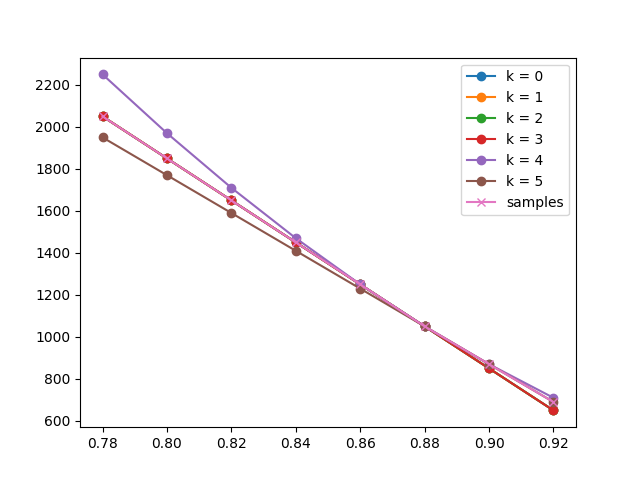
\includegraphics[width=\linewidth]{figures/figure1.png}
	\caption{Gráfica polinomios orden 2 y la muestra}
	\label{fig:interp_cuad}
\end{figure}

Se puede ver claramente que los polinomios tienen menor divergencia con los datos alrededor del punto 0.88.



Lo siguiente es ver cual polinomio ($P(x)$) tiene menor desviación.

Para ello calcularemos el RMSE (root mean square error) y el MAE (mean average error): 

\begin{equation}
	RMSE = \sqrt{ \frac{1}{N} \sum_{k=0} (y_k - p_k)^2 }
\end{equation}

\begin{equation}
	MAE = \frac{1}{N} \sum_{k=0} |{y_k - p_k}|
\end{equation}

donde:
$$ p_k = P(x_k) $$



\begin{table}[htbp]
	\centering
	\csvreader[
	tabular=|c|c|c|,
	table head=\hline \textbf{\#} & \textbf{RMSE} & \textbf{MAE}\\\hline,
	late after last line=\\\hline,
	]{data/errors01.csv}{}{\csvlinetotablerow}
\end{table}


\paragraph{}
Vemos que el polinomio con menor desviación es el polinomio de orden 2 que inicia en k = 1. 


\subsubsection{Resultado}

Generamos la edad estimada por cada polinomio para el valor $0.8705$. 

\begin{table}[htbp]
	\centering
	\csvreader[
	tabular=|c|c|,
	table head=\hline \textbf{\#} & \textbf{Age} \\\hline,
	late after last line=\\\hline,
	]{data/age01.csv}{}{\csvlinetotablerow}
\end{table}

Esto nos da que la edad estimada por el polinomio $P_1$ es:

$$
	P_1(0.8705) = 1144.999999999999 \approx{1145}
$$


\newpage

% ejercicio B

\section{Problema B - Propagación de errores}

Utilizando la propagación de errores estudiada en la asignatura de Técnicas
Experimentales I calcule el error asociado a la estimación de la edad obtenida en
el apartado anterior. Analice el resultado en relación a la tabla.


\subsubsection{Resolución}

Ver apartado anterior.
\newpage

% ejercicio C
\section{Problema C - Estimación mediante polinomios cúbicos}

Determine ahora una estimación de la edad de la muestra utilizando un polinomio de interpolación cúbico hacia adelante utilizando como punto de partida el dato correspondiente a i = 2. Presente también la expresión explícita del polinomio interpolador. Repita este apartado utilizando otro polinomio de interpolación cúbico hacia adelante con punto de partida i = 3. Utilice para ambos casos el método del interpolador de Lagrange.

\subsection{Resolución}

\subsubsection{Programación}

\paragraph{Generación de polinomios} Los polinomios de orden 3 se generan con el código descrito en \ref{gen_polynomials}:

\lstinputlisting[language=Python, firstline=47, lastline=64]{../../code/methods/lagrangian_interpolation.py}

Esto nos dará cinco polinomios, de los cuales solo usaremos dos, como en el siguiente snippet del código de los ejercicios.

\lstinputlisting[language=Python, firstline=16, lastline=16]{../../code/pecs/pec3/ex3.py}

\newpage 

\subsubsection{Polinomios generados vs muestras}

Una vez obtenidos los polinomios, pasamos a visualizarlos gráficamente.

\begin{figure}[H]
	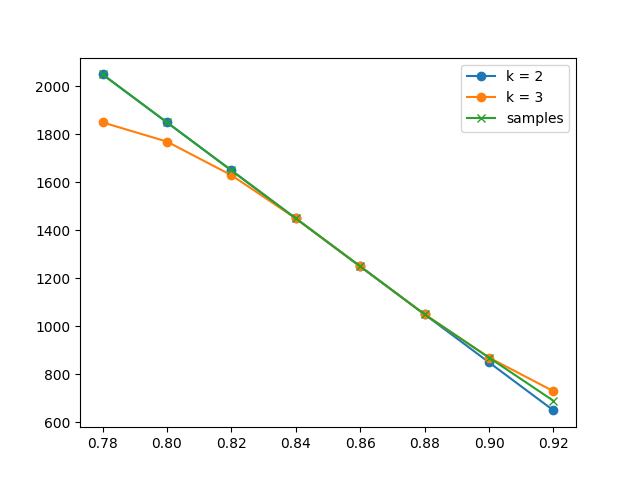
\includegraphics[width=\linewidth]{figures/figure2.png}
	\caption{Gráfica polinomios orden 3 y la muestra}
	\label{fig:interp_cub}
\end{figure}

Como es de esperar, vemos que los polinomios concuerdan más que nada en el rango que se usó para generar los polinomios (en especial a partir de k = 3).

\newpage 
\paragraph{} 
Esto queda ilustrado en la siguiente figura, donde vemos la diferencia entre los dos polinomios. 

\begin{figure}[H]
	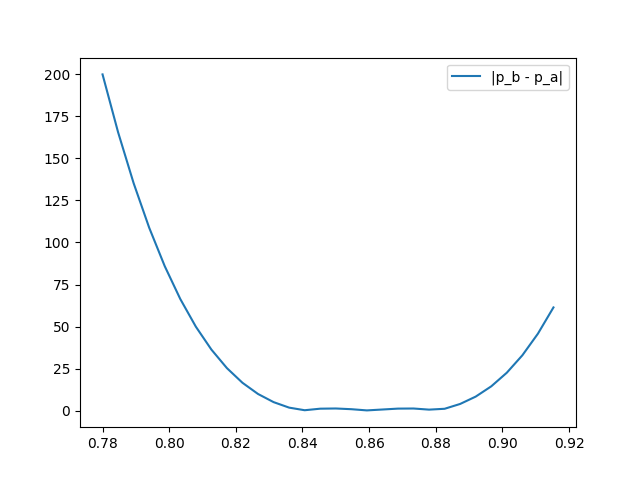
\includegraphics[width=\linewidth]{figures/figure3.png}
	\caption{Diferencia de los polinomios cúbicos}
	\label{fig:diff_interp_cub}
\end{figure}


\subsubsection{Resultados} 

Las edades interpoladas con los dos polinomios cúbicos ($k=2$, $k=3$) se ven en la siguiente tabla.

\begin{table}[htbp]
	\centering
	\csvreader[
	tabular=|c|c|c|,
	table head=\hline \textbf{\#} & \textbf{Age} \\\hline,
	late after last line=\\\hline,
	]{data/age02.csv}{}{\csvlinetotablerow}
\end{table}


\newpage

% ejercicio D
\section{Problema D - Estimación mediante diferencias progresivas de Newton}

Reproduzca el apartado anterior utilizando el método de las diferencias progresivas de Newton. Compare los resultados obtenidos y extraiga las conclusiones.


\subsection{Análisis}

\subsubsection{Teoría}

\paragraph{Definición}
El método de las diferencias progresivas de Newton es el siguiente.

Dado una serie de datos:

$$ S = \{ x_k, y_k \}^n $$

Se definen los polinomios base como: 

\begin{equation}
	n_k(x) = \prod_{j=0}^{k-1} (x - x_j) 
\end{equation}

con $n_0(x) = 1$.

El polinomio de interpolación es la combinación lineal de los polinomios base:

\begin{equation}
	N(x) = \sum_{k=0}^{n} [y_k] n_k(x)
\end{equation}

donde $[y_k]$ es la diferencia dividida.
\newpage

\subsection{Resolución}

\subsubsection{Programación}

\paragraph{Generación de polinomios} Los polinomios de orden 3 se generan con el código (muy similar al de lagrange):

\lstinputlisting[language=Python, firstline=4, lastline=37]{../../code/methods/newton.py}

Esto nos dará cinco polinomios, de los cuales solo usaremos dos, como en el siguiente snippet del código de los ejercicios.

\lstinputlisting[language=Python, firstline=16, lastline=16]{../../code/pecs/pec3/ex4.py}


\newpage 

\subsubsection{Polinomios generados vs muestras}

Una vez obtenidos los polinomios, pasamos a visualizarlos gráficamente.

\begin{figure}[H]
	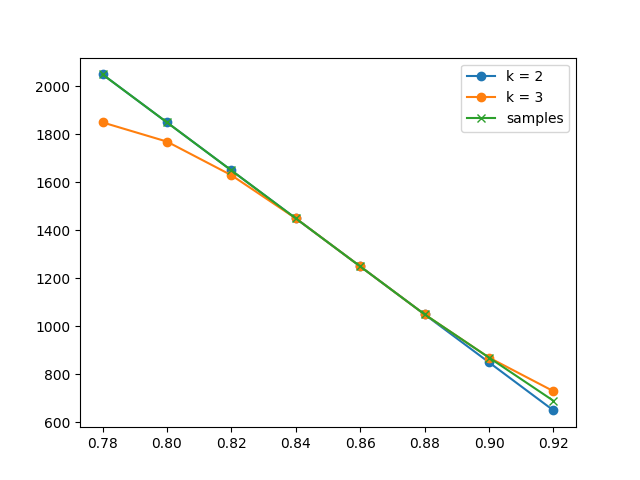
\includegraphics[width=\linewidth]{figures/figure4.png}
	\caption{Gráfica polinomios newton y la muestra}
	\label{fig:interp_newt}
\end{figure}



\newpage 
\paragraph{} 
Esto queda ilustrado en la siguiente figura, donde vemos la diferencia entre los dos polinomios. 

\begin{figure}[H]
	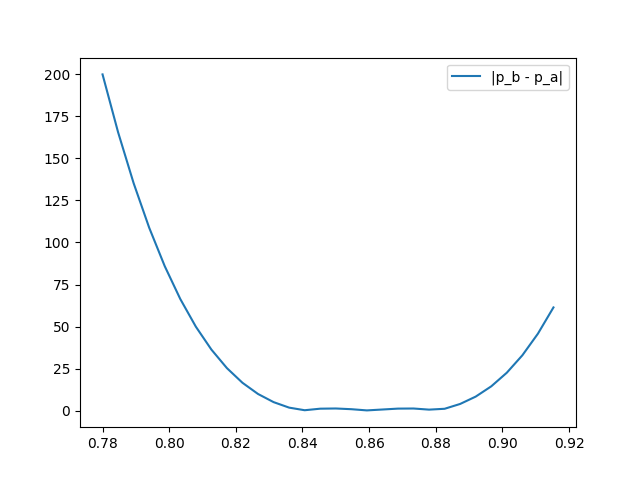
\includegraphics[width=\linewidth]{figures/figure5.png}
	\caption{Diferencia de los polinomios de newton}
	\label{fig:diff_interp_newt}
\end{figure}


\subsubsection{Resultados} 

Las edades interpoladas con los dos polinomios de newton ($k=2$, $k=3$) se ven en la siguiente tabla.

\begin{table}[htbp]
	\centering
	\csvreader[
	tabular=|c|c|c|,
	table head=\hline \textbf{\#} & \textbf{Age} \\\hline,
	late after last line=\\\hline,
	]{data/age03.csv}{}{\csvlinetotablerow}
\end{table}

\paragraph{Discusión} 
Los dos métodos para interpolar dan resultados idénticos en este contexto, por lo cual la elección de cual usar dependería del caso. Una ventaja del método de Newton es que si esperamos tener más muestras no habría que recalcular todo (con ligeras modificaciones el código podría reflejar esto).
\newpage

% ejercicio E
\section{Problema E - Error absoluto cometido}

\paragraph{Ecuación}
La antigüedad de la muestra es dada por:

\begin{equation}
	t = - \ln (N_{14C}) \frac{t_{12}}{\ln 2}
\end{equation}

y $t = 5730$



Estime el error absoluto cometido con las aproximaciones obtenidas en los 
apartados A) y C) y D) en relación a la edad t dada por expresión anterior. 

Realice una discusión sobre los órdenes de magnitud de los errores calculados.

\subsection{Resolución}

\subsubsection{Programación}
Si usamos la ecuación, vemos que la edad es: $1146.480157$.

Utilizaremos el siguiente código para calcular el error:

\lstinputlisting[language=Python]{../../code/pecs/pec3/ex5.py}

\newpage 

\subsubsection{Resultados}

Con esto tenemos los resultados en la siguiente tabla:

\begin{table}[htbp]
	\centering
	\csvreader[
	tabular=|c|c|c|,
	table head=\hline \textbf{Polynomial} & \textbf{Age} & \textbf{Error} \\\hline,
	late after last line=\\\hline,
	]{data/errors04.csv}{}{\csvlinetotablerow}
\end{table}

\subsection{Discusión}

Como se puede ver, el error es dos órdenes de magnitud por debajo del valor, lo cual es una aproximación relativamente buena.
\newpage

% ejercicio F
\section{Problema F - Regla del término siguiente}
Utilizando la regla del término siguiente estime el error cometido al datar la muestra cuya proporción de Carbono-14 es $0.8705$ con las aproximaciones calculadas en el apartado C) y D).

\subsection{Análisis}

La regla del término siguiente se basa en aproximar el error definiéndolo como la diferencia entre el polinomio de orden $n$ y el polinomio de orden $m = n + 1$.

Básicamente es el valor del término $m = n + 1$.


$$ E_{sig}(x)_n = P_{n+1}(x) - P_{n}(x) $$

\subsection{Resolución}

\subsubsection{Programación}

Utilizaremos el siguiente código para calcular el error:

\lstinputlisting[language=Python]{../../code/pecs/pec3/ex6.py}

\newpage 

\subsection{Resolución}

Los errores de cada orden, para el valor de interés $0.8705$ se han calculado:

\begin{table}[htbp]
	\centering
	\csvreader[
	tabular=|c|c|c|,
	table head=\hline \textbf{Polynomial} & \textbf{Error} \\\hline,
	late after last line=\\\hline,
	]{data/errors05.csv}{}{\csvlinetotablerow}
\end{table}


\newpage 

% ejercicio G
\section{Problema G - Error de la interpolación}\label{sec:interp_err}

Se define el error de una interpolación como
$$E(x) = \frac{ f^{n+1}(\xi) }{ (n+1)! } \prod_{i=0}^{n}(x - x_i) $$

donde $n$ es el grado del poliniomio interpolante, $f^{(n+1)}$ la derivada $n+1$ de la función y $\xi$ pertenece al intervalo que contiene todos los puntos utilizados. 

Represente gráficamente, en el intervalo adecuado y para las aproximaciones del apartado C) y D), las funciones de error dadas por la fórmula anterior usando aquellos valores
de $\xi$ que, dentro del intervalo considerado, la maximizan y la minimizan. Obtenga también las cotas de error que podemos extraer para esas aproximaciones.

\subsection{Resolución}

Primero tomaremos las primeras cuatro derivadas:

\begin{align}
	\partial_{\mu} f(\mu)
	&= - \frac{1}{\mu} C  \\
	\partial_{\mu}^{2} f(\mu)
	&= \frac{1}{\mu^2} C \\
	\partial_{\mu}^{3} f(\mu)
	&= \frac{-2}{\mu^3} C \\
	\partial_{\mu}^{4} f(\mu)
	&= \frac{6}{\mu^4} C	
\end{align}
\newpage

\subsubsection{Error cuadrático}

El error en la aproximación cuadrática es dado por la función:

$$ E_{cuad} = \frac{ \partial_{\mu}^3(\xi) }{3!} \prod_{i=0}^{2} (x - x_i) $$

Queremos encontrar pues, dos $\xi$ tal que $\partial_{\mu}^3(\xi)$ sea máxima o mínima en el intervalo $[0.78, 0.92]$.

\paragraph{Valores $\xi_{min}, \xi_{max}$}

Encontrar los valores $[\xi_{min}, \xi_{max}]$ no es tan complicado si observamos que se trata de $\partial_{\mu}^3(\xi) \approx -2\mu^{-3} $. Por ende los extremos del intervalos son también los extremos de $\partial_{\mu}^3(\xi)$ en ese intervalo.

\paragraph{Resultado}


A continuación se han visualizado la función de error para los dos valores de $[\xi_{min}, \xi_{max}]$. Como se puede ver, el error es de magnitud bastante inferior al rango de interés (miles de años).


\begin{figure}[H]
	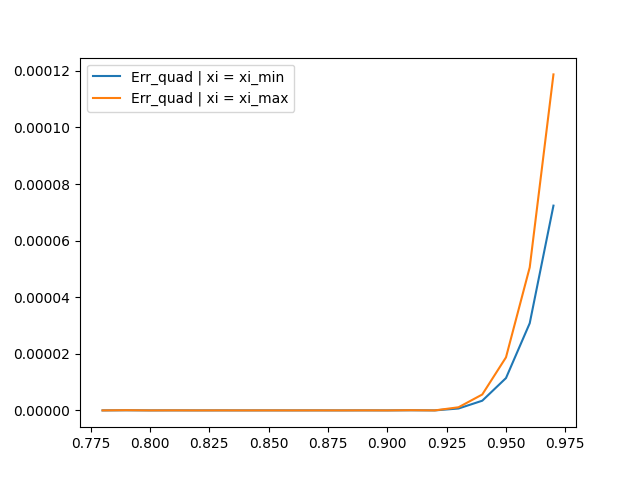
\includegraphics[width=\linewidth]{figures/figure6.png}
	\caption{Error en la aproximación cuadrática}
	\label{fig:err_cuad}
\end{figure}


\subsubsection{Error cúbico}

El error en la aproximación cúbica es dado por la función:

$$ E_{cub} = \frac{ \partial_{\mu}^4(\xi) }{4!} \prod_{i=0}^{3} (x - x_i) $$

Queremos encontrar pues, dos $\xi$ tal que $\partial_{\mu}^4(\xi)$ sea máxima o mínima en el intervalo $[0.78, 0.92]$.

Seguiremos una metodología parecida a la sección anterior.

\paragraph{Valores $\xi_{min}, \xi_{max}$}

Encontrar los valores $[\xi_{min}, \xi_{max}]$ no es tan complicado si observamos que se trata de $\partial_{\mu}^4(\xi) \approx 6\mu^{-4} $. Por ende los extremos del intervalos son también los extremos de $\partial_{\mu}^3(\xi)$ en ese intervalo.

\paragraph{Resultado}

A continuación se han visualizado la función de error para los dos valores de $[\xi_{min}, \xi_{max}]$. Como se puede ver, el error es de magnitud bastante inferior al rango de interés (miles de años).

\begin{figure}[H]
	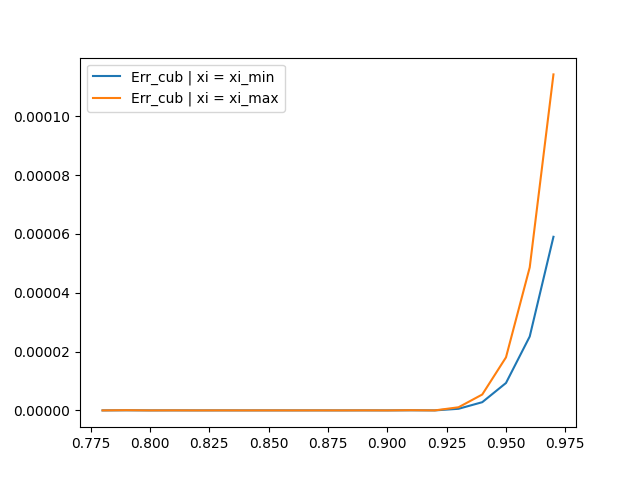
\includegraphics[width=\linewidth]{figures/figure7.png}
	\caption{Error en la aproximación cúbica}
	\label{fig:err_cub}
\end{figure}


\newpage

\subsubsection{Código}

El código utilizado para este ejercicio es:

\lstinputlisting[language=Python]{../../code/pecs/pec3/ex7.py}




\newpage

\subsubsection{Discusión}


Como se puede ver, los polinomios de orden $n = 2$ y $n = 3$ dan resultados similares. 

Los errores calculados son:

\begin{table}[htbp]
	\centering
	\csvreader[
	tabular=|c|c|c|,
	table head=\hline \textbf{Error} & \textbf{Value} \\\hline,
	late after last line=\\\hline,
	]{data/errors06.csv}{}{\csvlinetotablerow}
\end{table}

\paragraph{Error relativo}
Los valores aproximados estan en el orden de $f(x) \approx 10^{3}, ~ \forall x \in [0.78, 0.92]$. Considerando que el error de aproximación se ha visto que está por el orden de $E(x) \approx 10^{-9}, ~ \forall x \in [0.78, 0.92]$.

\subparagraph{Magnitud}

La magnitud del error relativo es aproximadamente:

\begin{align*}
	\frac { E(x) } { f(x) } 
	&\approx \frac{10^{-9}}{10^3}
	= 10^{-12}
\end{align*}

Lo que nos inspira bastante confianza en la edad obtenida por la interpolación.

\paragraph{Selección de datos}
Si nos encargamos de que los polinomios se construyan con los datos mas cercanos de los puntos de interés, podremos tener una aproximación relativamente buena.


Una buena manera de entender esto es ver que la interpolación de Lagrange usa la información contenida en un intervalo, que contrasta con otras formas de aproximar una función como la aproximación por polinomios de Taylor, donde la información se encuentra en el punto y las derivadas de $x$.


\newpage 

% ejercicio H
\section{Problema H - Discusión de errores}

Discuta los órdenes de magnitud de los errores calculados en los apartados E) y F) para los polinomios interpolantes cúbicos, en particular, razone si influye en el error la elección de unos datos u otros para interpolar.

\subsubsection{Resolución}

Ver apartado \ref{sec:interp_err}.
\newpage 

% ejercicio I
\section{Problema I - Discusión de errores pt. 2} 

Indique si estos errores, para el valor de la proporción $N_{14C}$ es 0.8705, se encuentran entre los valores máximo y mínimo calculados usando la expresión $E(x)$.

\subsubsection{Resolución}

Ver apartado \ref{sec:interp_err}.
\newpage 

% ejercicio J
\section{Problema J - Discusión General}

Realice finalmente una discusión general de los resultados obtenidos en los
distintos apartados para la datación de la muestra, en términos de la magnitud y el error asociado. Compare los resultados obtenidos matemáticamente con los criterios de la estimación de medidas y errores aprendidos en la asignatura de Técnicas Experimentales I.

\subsection{Resolución}

Ver apartado \ref{sec:interp_err}.
\newpage 


\end{document}
